# Analysis

## Exploratory Data Analysis
Before building our model, we first wanted to understand the data that we were building our model on. Below, I've shown the summary statistics for the quantitative variables in our model. 

### Quantitative variables
Summary Statistics of Quantitative Variables
Min, 1st Quartile, Median, Mean, 3rd Quartile, Max of quantitative variables
\input{quantitative_summary, file = '../../data/eda.txt'}
Range of Quantitative Variables
\input{quantitative_range, file = '../../data/eda.txt'}
IQR of Quantitative Variables
\input{quantitative_IQR, file = '../../data/eda.txt'}
Standard Deviation of Quantitative Variables
\input{quantitative_SD, file = '../../data/eda.txt'}

I've also attached histograms below, which describe the distributions of some of the more relevant quantitative variables. 

Histogram
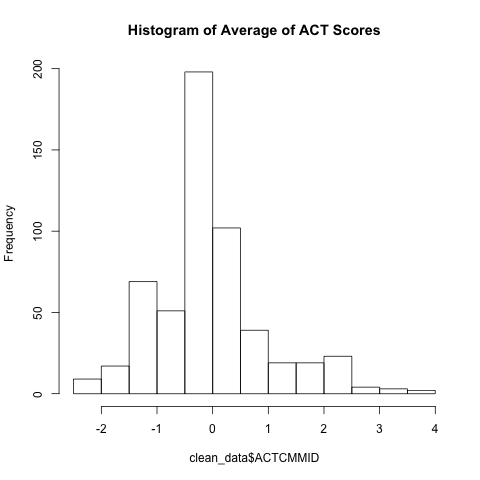
\includegraphics{../../images/histogram_ACT_avg.png}
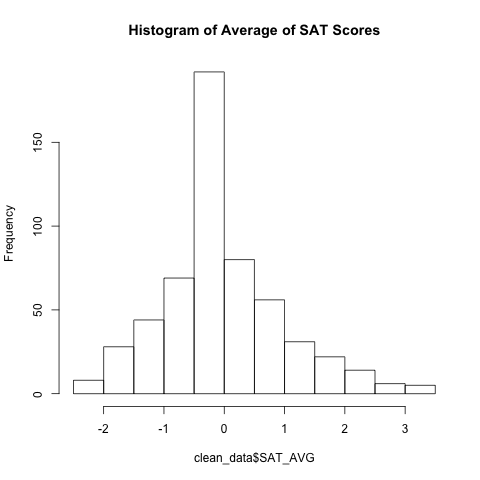
\includegraphics{../../images/histogram_SAT_avg.png}

\includegraphics{../../images/histogram_majors.png}
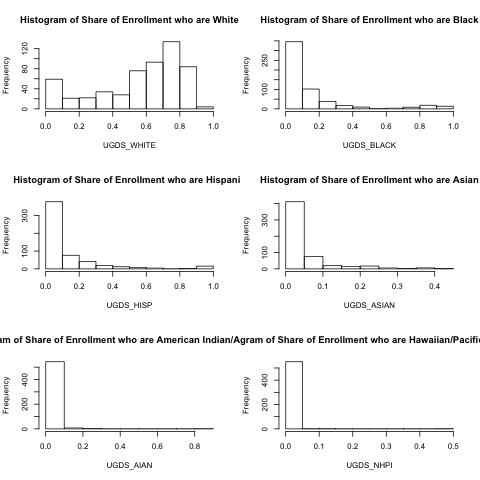
\includegraphics{../../images/histogram_race_enrollment.png}
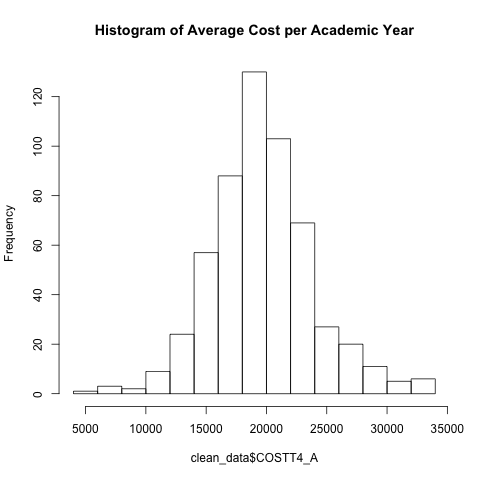
\includegraphics{../../images/histogram_net_price.png}
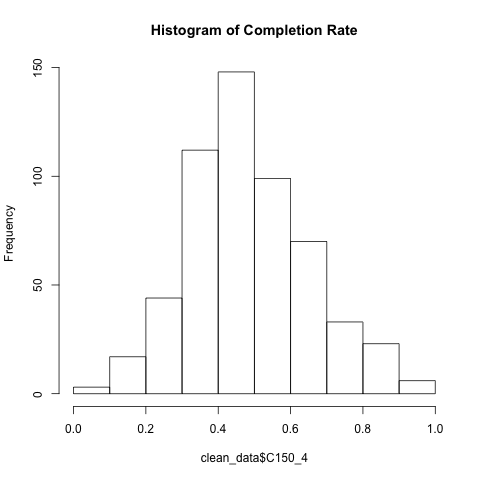
\includegraphics{../../images/histogram_completion.png}
\includegraphics{../../images/histogram_income_graduation.png}
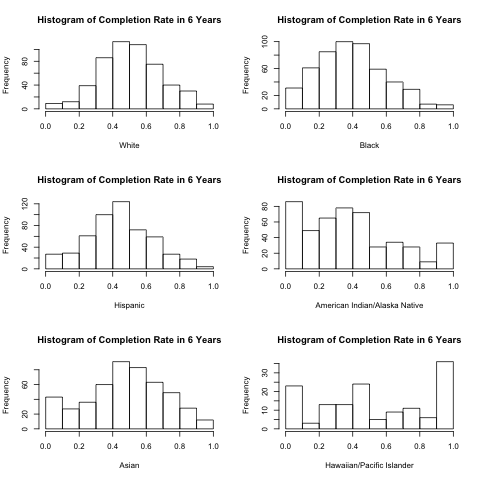
\includegraphics{../../images/histogram_race_completion}
